This section discusses the sources of the estimated gender differences. A major determinant is the choice of the alternative childcare arrangements. Estimated treatment effects are very similar across genders comparing treatment to staying at home full time. Males benefit much more from treatment relative to low-quality childcare compared to treatment relative to staying at home. This result is consistent with previous research that shows (i) substantial gender differences resulting from attending low-quality childcare \citep{Kottelenberg-Lehrer_2014_Gender-Effects,Baker_Gruber_Milligan_2015_Noncog_Defects}; and (ii) that females are less sensitive to more stressful, low quality environments (see, e.g., \citealp{golding2016psychology,Autor-etal_2015_Family-Disadvantage}).

Table~\ref{tab:proportion-table-ranksign} shows the proportion of outcomes by category for which male outcomes exceed those of females. In Appendix~\ref{appendix:propmales-females}, we present analogous tables for staying at home and attending alternative preschool. We also partition the sample by father's presence, a potentially important moderator.\footnote{Recall that we condition on baseline variables to control for selection into childcare for controls. See Appendix~\ref{appendix:amethodology} for a sensitivity study using other methods. They produce comparable estimates, but are less precisely estimated.} Figure~\ref{fig:proportion-altpre} shows the proportions partitioned by alternative childcare setting. The males who stay at home do better than the females in cognitive and parenting measures, employment, and across all outcomes. Unlike the males who attend lower-quality alternative preschool, the males who stay at home have similar crime outcomes as the females. Given the important negative effects of male criminal activity, this finding highlights the magnitude of harm caused by low-quality alternative preschools for males.

\begin{figure}[H]
\centering
\caption{Proportion of Outcomes Males $>$ Females, by Outcome Category, Partitioning by Alternative Childcare Setting}
\label{fig:proportion-altpre}
	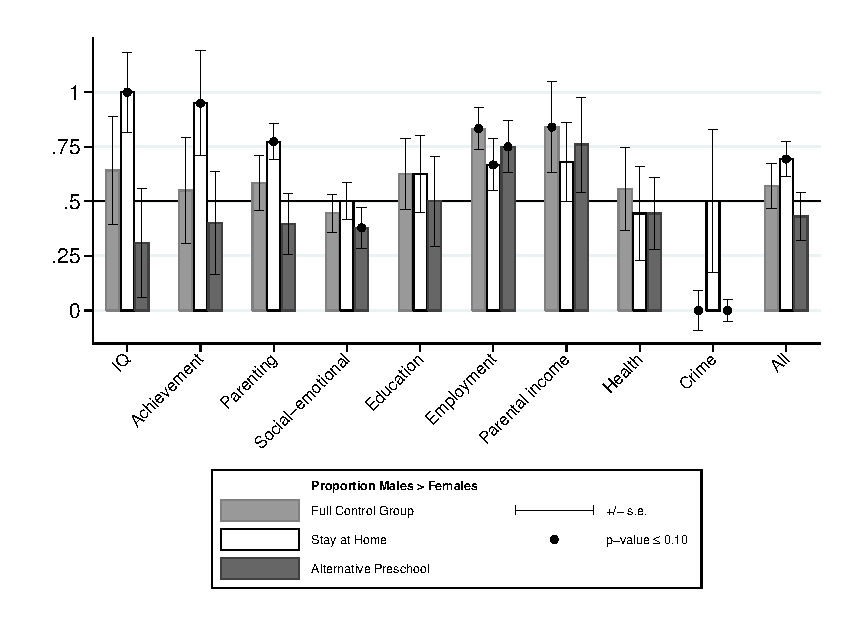
\includegraphics[width=\textwidth]{output/gendergaps-control-moderated-altpre}
\footnotesize \justify
Note: These plots show the proportion of outcomes, by outcome category, for which the males' mean is larger than the females' mean. The standard errors and the $p$-values are computed using 1,000 bootstraps. The $p$-values are one-sided and test the null hypothesis that the proportion of outcomes is greater than 50\% All outcome categories have higher values corresponding to socially desirable outcomes.
\end{figure}

Appendix~\ref{appendix:genderdifferences} reports estimates by whether or not the father is present (Figure~\ref{fig:proportion-fhome}). Parenting is better for control-group males when the father is absent. While this may seem contradictory, the parenting measure includes a scale that captures the absence of punishment. Control-group males with an absent father tend to have higher parenting scores, especially for this scale, relative to control-group males with a father present. In the treatment group, the males with a present father do better than those with an absent father. This hints at a complementarity between the father's parenting and the high-quality treatment. Besides this, few clear-cut patterns emerge. Father's presence interacted with treatment also favors males for IQ. Males in the control group do better when the father is absent in employment.

Another measure of home environment is maternal locus of control which is measured when the subjects were 1.5 years old.\footnote{See \citet{Rotter_1966_PMGaA}. The researchers implementing ABC/CARE slightly modified the scale to be more appropriate for the population.} An internal locus of control, which is socially desirable, indicates feelings that the respondents can control future outcomes. In contrast, an external locus of control indicates feeling that outside forces determine future outcomes (e.g. luck). We consider pairs of opposing statements. The respondent chooses the statements that more closely align with her beliefs. One point is given for each statement the respondent selects that corresponds with an external locus of control. An example is: ``In the long run people get the respect they deserve in this world'' versus ``Unfortunately, an individual's worth often passes unrecognized no matter how hard he tries.'' If the respondent selects the second statement, she has a greater perception of external locus of control.  We define a respondent as having an internal locus of control if they score below the sample mean and as having an external locus of control if they score at or above the sample mean.

Figure~\ref{fig:proportion-mlocus} shows the proportion of outcomes by category that favor males classified by locus of control. In the control group, a higher internal maternal locus of control promotes better outcomes for males across all outcome categories except health. Another way to state this is that males are more negatively affected if their mothers have a higher external locus of control than are females. This is consistent with the analyses of \citet{Schore_2017_IMHJ} and \citet{golding2016psychology}. Although locus of control does not necessarily measure depression, this finding is consistent with \citet{Beeghly-etal_2017_IMHJ}, who finds that increased maternal depression leads to worse outcomes for young males relative to females.

\begin{figure}[!htbp]
\centering
\caption{Proportion of Outcomes Males $>$ Females, by Outcome Category, Dividing by Maternal Locus of Control}
\label{fig:proportion-mlocus}
\begin{subfigure}[h]{0.7\textwidth}
	\centering
	\caption{Control Group}
	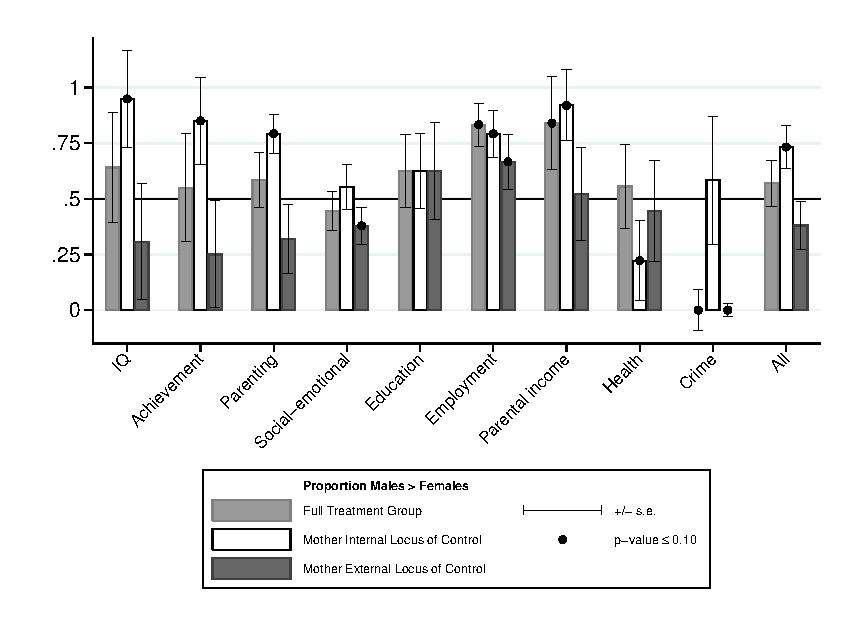
\includegraphics[width=\textwidth]{output/gendergaps-control-moderated-mlocus}
	\end{subfigure}
	
\begin{subfigure}[h]{0.7\textwidth}
	\centering
	\caption{Treatment Group}
	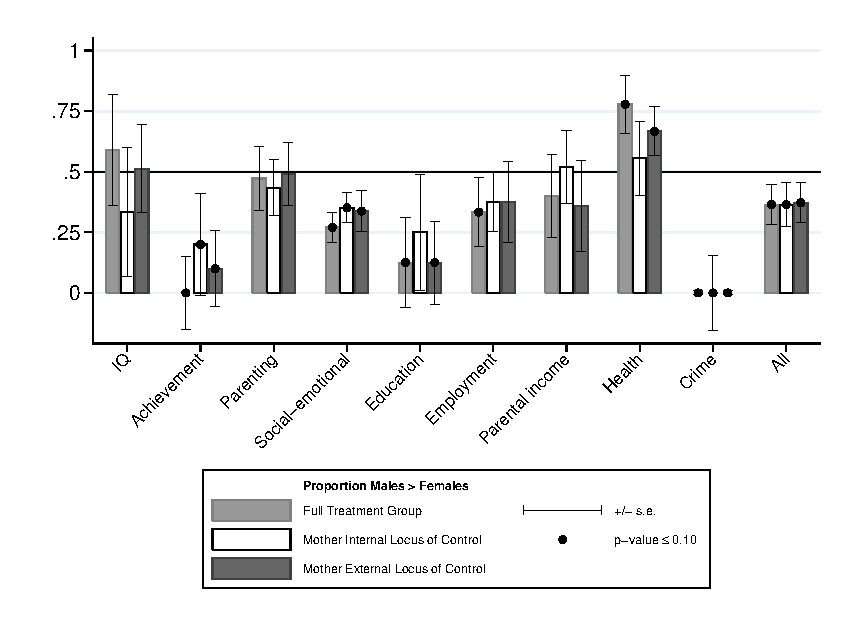
\includegraphics[width=\textwidth]{output/gendergaps-treatment-moderated-mlocus}
	\end{subfigure}
\footnotesize \justify
Note: These plots show the proportion of outcomes, by outcome category, for which the males' mean is larger than the females' mean. The standard errors and the $p$-values are computed using 1,000 bootstraps. The $p$-values are one-sided and test the null hypothesis that the proportion of outcomes is greater than 50\%. All outcome categories have higher values corresponding to socially desirable outcomes.
\end{figure}

Maternal locus of control moderates treatment outcomes differently. Aggregating across outcomes, male treatment outcomes are not much affected by the mother's locus of control. Outcomes are affected for those in the control group. This is especially strong for mental health outcomes. The reduced differential in the treatment group suggests an important compensating role of enriched early childhood programs.



